\chapter{Strängars rörelse i vätskor}

%\subsubsection{Strängrörelser inom cellen}
Aktinfilament är polymerer vilka utgör en viktig byggsten för cellens cytoskelett och transportväg för motorprotein vilka formar och bidrar till cellens utseende, dynamik och stadga. För att kunna ge en mer detaljerad beskrivning av dessa egenskaper är studien av enstaka aktinfilaments dynamik av stort intresse. I detta arbete har olika dynamiska egenskaper för aktinfilament studerats, både för filament som fluktuerar fritt i en vätska och filament instängda i en rektangulär kvasi-2D mikrokanal. Mikrokanalen är till för att simulera beteendet hos aktinfilament i cytoskelettet där det omges av andra filament och därmed har en begränsad möjlighet till rörelse.

%\section{}


\section{Modeller för strängrörelser}
Aktinfilamenten precis som tidigare studerade partiklar påverkas av diffusionsprocessen inuti celler och således krävs stokastiska modeller för att beskriva rörelsen. En vanligt använd modell inom polymerfysiken är Worm Like Chain-model som beskrivs nedan. Vidare studeras en modell i form av en langevinekvation med en brusterm som innehar brownsk karaktär.

\subsection{Worm Like Chain-model}
Worm like chain modellen \cite{Milstein2013} (WLC) är en modell som ämnar beskriva fluktuationerna hos en semi-flexibel polymer. I modellen antas att polymeren är helt oelastisk, enbart påverkas av termiskt brus och styv på små längdskalor. Då polymeren fluktuerar fritt utan att vara instängd i en mikrokanal ges en minimalistisk WLC beskrivning av att filamentets fluktuationer regleras av böjningsenergin. För en polymer av $N$ segment vardera med riktning \textbf{r}$_i$ och längd $\abs{r_{i}}=l$ samt polymerens böjstyvhet $\kappa$ ges böjningsenergin av 
\begin{equation}
    H = -\kappa\sum_{i=1}^{N}\textbf{r}_{i}\cdot \textbf{r}_{i+1}.
\end{equation}
Maximalt bidrag till energin från två på varandra följande segment fås alltså om dessa har antiparallell riktning. Givet identiteten $\textbf{r}_{i}\cdot\textbf{r}_{i+1}=\frac{2l^2-(\textbf{r}_{i+1}-\textbf{r}_{i})^2}{2}$ kan summan skrivas om som en integral i gränsen då $N \rightarrow \infty$, $\kappa\to\infty$, $l \rightarrow 0$ samt produkten \todo{Någon annan variabelnamn än $\xi$?}$\kappa l=\xi$ finit 
\begin{equation}\label{böj}
    H=\frac{\xi}{2}\int_{0}^{L}ds(\partial_{s}\textbf{t}(s))^2,
\end{equation}
där $\textbf{t}(s)$ är enhetstangentvektorn längs polymeren parametriserad med båglängden. Detta är den kontinuerliga WLC modellen \cite{Fixman_WLC1973} vilket ger en bra approximation av en polymer där längden hos enstaka molekyler kan försummas. \todo{Den diskreta modellen heter väl FJC=freely jointed chain? Inte diskret WLC?} Korrelationen mellan två tangentvektorer medelvärdsbildat över tid ges av \cite{Landau1958}:
\begin{equation}
\ev{\textbf{t}(s)\textbf{t}(s+\Delta s)}=e^{-\frac{\abs{\Delta s}}{2L_{p}}},
\end{equation}
där $L_{p}=\frac{\xi}{k_{B}T}$ är kvoten mellan styvheten hos polymeren och termiska energin hos fluiden. Denna kallas \emph{persistent length} och ger ett mått på hur snabbt tangentkorrelationen avtar längs polymeren. 

I fallet då $\nicefrac{L_{p}}{L}>1$ sägs polymeren vara styv. Ytterligare kan ett rumsligt medelvärde av dessa tangentkorrelationer beräknas. Beteckna denna rumsliga medelvärdesbildning med ett heldraget streck. Tangentkorrelationen beror då på avståndet mellan tangentvektorerna, $\Delta s$, och kan definieras som
\begin{equation}
\label{tangkorr}
    \ev{cos\theta(\Delta s)}\equiv\overline{\ev{\mathbf{t}(s)\mathbf{t}(s+\Delta s)}}.
\end{equation}
Denna minimalistiska WLC modell är intressant då den utgår från att strängen kan fluktuera fritt. Givet ett dataset av fria strängar samt strängar placerade i mikrokanaler kan dess påverkan på tangentkorrelationen studeras. Då en sträng i en mikrokanal antas uppleva en återställande kraft riktad mot centrum av kanalen väntas dess tangentkorrelation vara mer ihärdig.

\subsection{WLC-modell för sträng i mikrokanal}

En mer sofistikerad modell kan konstrueras med avseende till mikrokanalens egenskaper och dess dynamik. Då interaktionen mellan strängen och kanalens väggar beskrivs som rent sterisk \cite{Koster_etal2007} kan denna approximeras med en parabolisk potential. Därmed införs kraften $F \propto A(s)^2$ där $A(s)$ svarar mot strängens avstånd vinkelrätt centrum av kanalen. Potentiella energin för denna kraft blir
\begin{equation}
    H_{pot}=\int_{0}^{L} ds[\gamma z(s)^2],
\end{equation}
där $\gamma$ är en positiv konstant vars storlek avger styrkan hos potentialen. 

Då tangentvektorn till strängen kan defineras som $\mathbf{t}(s)=\partial_sA(s)$ fås hamiltonianen för systemet som summan av de potentiella energierna

\begin{equation}
\label{Htot}
    H_{tot}=\int_{0}^{L}ds[\xi\partial_{s}^{2}A(s)^2 + \gamma A(s)^2].
\end{equation}

Där första termen i integranden svarar mot energin enligt den tidigare modellen \eqref{böj} uttryckt i strängens avstånd från centrum av kanalen.

Hamiltonianen ger alltså en modell av kraften verkandes på en sträng i en mikrokanal \todo{inte riktigt rätt}. Det ses att energin för en sträng minimeras i fallet då den är helt rak och fixerad längs centrum av kanalen. Kraften återställer alltså eventuella avvikelser från kanalens centrum. Då avvikelserna uppstår på grund av termiska fluktuationer, vilket antas vara stokastiska, kan som tidigare i \ref{brownsk} systemet betraktas med en langevinekvation. Då strängens intrinsiska tröghet, svarandes mot högre ordningens tidsderivata, försummas fås\cite{PhysRevE.60.4671}
\todo{jobba på övergången}

\begin{equation}
\label{mans}
    \partial_{t}A(t,s)=-\gamma A(t,s)+\xi \partial_{x}^{2}A(t,s)+\sigma \partial_{t}W(t,s).
\end{equation}
Där fluktuationera approximerats med termen $W(t,s)$, ett stokastiskt vitt brus vars intensitet är proportionellt mot $\sigma$. Notera hur langevinekvationen även beskriver tidsutveckling av systemet.

\todo{kanske en subsection här}

Definera fouriertransformation som
\begin{equation}
    \hat{A}(t,k)=\int_{-\infty}^{\infty}\dd{s} A(t,s)\ee^{-\ii sk}
\end{equation}
Genom fouriertransformation av \eqref{mans} fås en ordinär stokastisk differentialekvation av första ordningen
\begin{equation}
        \partial_{t}\hat{A}(t,k)=-\left(\gamma+\xi k^2\right)\hat{A}(t,k)+\sigma \partial_{t}\hat{W}(t,k).
\end{equation}
Då $\zeta=\gamma+\xi k^2$ är denna ekvation ekvivalent med \todo{ref 3.26} vars lösning redan är känd. Kovariansen kan nu beräknas och på samma sätt som \todo{ref 3.28} fås
%\begin{equation}
%        \hat{A}(t,s)=\ee^{-(\gamma+\alpha s^2)t}\left(\hat{A}(0,s)+\sigma\int_{0}^{t}\dd\tau \ee^{(\gamma+\alpha s^2)\tau}\partial_{t}\hat{W}(\tau,z)\right)
%\end{equation}
%Tvåpunktskorrelationen för den fouriertransformerade stokastiska variabeln $\hat{A}(t,s)$ kan då beräknas till
\begin{equation}\label{jobbig}
\begin{aligned}
    \ev{\hat{A}(t,k)\hat{A}(t',k')} =& \ev{\hat{A}(0,k)\hat{A}(0,k')} \ee^{-(\gamma+\xi k^2)(t+t')}\\ 
    &+ \sigma^2 \int_{0}^{t}\int_{0}^{t'}\dd\tau\dd\tau' \ee^{(\gamma+\xi k^2)(\tau+\tau')} \ev{\partial_{t}\hat{W}(\tau,k)\partial_{t}\hat{W}(\tau',k')}.
\end{aligned}
\end{equation}
Notera att integralen beror på fouriertransformen av vitt brus $W(t,k)$. Denna kan beräknas genom fouriertransform av \todo{ref korr vitt brus} och följande resultat erhålls 
\begin{equation}
    \ev{\partial_{t}\hat{W}(t,k)\partial_{t}\hat{W}(t',k')}=\delta(t-t')\delta(k+k').
\end{equation}
Insättning av denna identitet i \eqref{jobbig} samtidigt som ekvationen betraktas i gränsen då $t,t'\rightarrow\infty$ medan $\Delta t=\abs{t-t'}$ hålls finit fås 
%\begin{equation}\label{jobbig}
%     \ev{\hat{A}(t,s)\hat{A}(t',s')}=\sigma^2\int_{0}^{t}\int_{0}^{t'}\dd\tau\dd\tau'\ee^{(\gamma+\alpha s^2)(\tau+\tau')}\ev{\partial_{t}\hat{W}(\tau,s)\partial_{t}\hat{W}(\tau',s')}.
%\end{equation}

%Då termiska bruset antas vara brownskt definieras det av följande tvåpunktskorrelation
%\begin{equation}\label{brus}
%    \ev{\partial_{t}W(t,z)\partial_{t}W(t',z')}=\delta(t- t')\delta(z-z')
%\end{equation}
%Fouriertransformation av \eqref{brus} ger \todo{ekvation 4.13+4.14 kanske kan skippas om man vill minska antal ekvationer.}
%\begin{equation}
%    \ev{\partial_{t}\hat{W}(t,s)\partial_{t}\hat{W}(t',s')}=\int_{-\infty}^{\infty}\int_{-\infty}^{\infty}\dd z \dd z'\ev{\partial_{t}W(t,z)\partial_{t}W(t',z')}\ee^{-izs}\ee^{-iz's'}
%\end{equation}
%\begin{equation}\label{fourbrus}
%    \ev{\partial_{t}\hat{W}(t,s)\partial_{t}\hat{W}(t',s')}=\delta(t-t')\int_{-\infty}^{\infty}\int_{-\infty}^{\infty}\dd z \dd z'\delta(z-z')\ee^{-i(sz+s'z')}=\delta(t-t')\delta(s+s')
%\end{equation}
\begin{equation}
    \ev{\hat{A}(t,k)\hat{A}(t',k')}=\frac{\sigma^2}{2(\gamma+\xi k^2)}\delta(k+k')\ee^{(\gamma+\xi k^2)\abs{t-t'}}.
\end{equation}
Slutligen återfås återfås kovariansen för de rumsliga variblerna $s$,$s'$ genom invers fouriertransform
\begin{equation}
\label{2korr}
    \ev{A(t,s)A(t',s')}=\frac{1}{(2\pi)^2\sqrt{\gamma\alpha}}\int_{-\infty}^{\infty}\dd p \frac{\ee^{-(1+p^2)\gamma \abs{t-t'}+\ii p\sqrt{\frac{\gamma}{\alpha}}(s-s')}}{1+p^2}.
\end{equation}

Där variabeln $p$ är en hjälpvariabel definerad som $\frac{dp}{dk}=\sqrt{\frac{\xi}{\gamma}}$. Då det ses att kovariansen enbart beror på differensen mellan variablerna $t$,$t'$ samt $s$,$s'$ är denna translationsinvariant, dvs $\ev{A(t,s)A(t',s')}=\ev{A(t+\delta t,s)A(t'+\delta t,s')}$. Därmed ges systemets tvåpunktkorrelation av
\begin{equation}
    c(\Delta t,\Delta s)=\frac{\ev{A(\Delta t,\Delta s)A(0,0)}}{\ev{A(0,0)A(0,0)}}.
\end{equation}

Tolkningen av tvåpunktskorrelationen är att ge mått på hur snabbt avvikelser från strängens jämviktsläge skingras med tiden samt avstånd på strängen. Givet data från strängar begränsade av en 2D-mikrokanal kan tvåpunktskorrelationen beräknas numeriskt och de fysikaliska parametrarna $\xi,\gamma,\sigma$ kan bestämmas. 

Tvåpunktskorrelationen kan även betraktas i fallet då $\abs{t-t'}\equiv 0$, vilket likt den minimalisktiska WLC modellen svarar mot korrelation längs strängen. \eqref{2korr} kan i detta fallet lösas helt analytiskt
\begin{equation}
\ev{A(z)A(z')}=\exp(-\sqrt{\frac{\gamma}{\xi}}\abs{\Delta s}).
\end{equation}
Motsvarande Persistent length för en sträng i en mikrokanal kan definieras som $L_{p}=\sqrt{\frac{\alpha}{\gamma}}$.



\section{Egenmoder}
Ett vanligt sätt att studera svängningar är att dela upp svängningarna i egenmoder. Genom en linjärkombination av dessa egenmoder kan en godtycklig svängning representeras. Anledningen till att det är intressant att studera egenmoder är på grund av att de är oberoende av varandra. Precis som \todo{beskriva mer tydligt hur data ser ut samt hur avst etc beräknas.} svängningen på en gitarrsträng kan strängens svängningar i cellen eventuellt representeras som en linjärkombination av dess egenmoder. 



Metoden för att åstadkomma denna sönderläggning av strängens rörelse i egenmoder beskrivs i avsnitt \ref{sec:kovmatris} som en diagonalisering av kovariansmatrisen, där kovariansmatrisen $C$ i detta fallet byggs upp av avståndskomponenter till strängen. Hädanefter betecknas därför det transversella avståndet till strängen relativt sitt jämviktsläge $A_s(t)$ där $s$ är en diskret båglängdsparameter längs med strängen. Diagonalisering av denna kovariansmatris med hjälp av spektralsatsen leder effektivt till ett basbyte från en bas bestående av det transversella avståndet i varje $s$ längs strängen, till en bas bestående av egenmoderna för strängen. Egenvärdena till kovariansmatrisen ger ett mått på hur mycket av strängens rörelse som byggs upp av motsvarande egenmod. Genom att projicera strängens rörelse på ett fåtal av de egenmoder med störst egenvärde förenklas analysen\cite{Shlens_PCA2014}; karakteristiska egenskaper för varje egenmod kan undersökas separat. 

\subsection{Transversella fluktuationer kring strängens jämviktsläge}
\todo[inline]{Detta ska nog så småningom ligga tidigare eftersom 5.1 också innefattas av detta. Eventuellt kanske det var delvis detta som var tänkt i appendix?}
Strängens rörelse parametriseras med båglängdsparametern $s\in[0,L]$ och ett polynom i $x$-led samt ett i $y$-led anpassas, proceduren bakom detta beskrivs i \ref{app:polynomanpassning}. I denna rapport har strängens translationsrörelse till stor del försummats genom att i varje tidpunkt placerat strängens masscentrum i origo. Givet detta är det intressant att studera huruvida strängarna fluktuerar kring något jämviktsläge.\todo{antyd att det gör det} En uppskattning av jämviktsläget $\mathbf{r}_0(s)$ tas fram genom att beräkna medelvärdespolynomet som representerar strängrörelsen. 

Från detta jämviktsläge har det transversella avståndet beräknats enligt 
\begin{equation}
A_s(t) = \mathbf{n}_0(s)\cdot\mathbf{r}(s,t),
\end{equation}\todo{Figur på detta kanske hade vart bra.}
där $\mathbf{n}_0(s)$ är en normerad normalvektor till strängens jämviktsläge och $\mathbf{r}(s,t)$ är avståndet till $s$ på strängen vid tid $t$ relativt $\mathbf{r}_0(s)$. I datan som analyserats i denna rapport är båglängdsparametern vald sådan att $s\in[0,L]$, där $L$ är strängens längd, och består av $n=\unit[128]{}$ diskreta ekvidistanta steg som representerar rörelsen. Kovariansmatrisen bildad av $A_s(t)$ kan bildas enligt \eqref{eq:kovmatris} som 
\begin{equation}
\label{eq:C}
    C_{ij} = \COV{A_s(t)}{A_{s'}(t)}_t.
\end{equation}
Egenvektorerna till $C$, hädanefter egenmoderna, betecknas $\mathbf{B}_i$ och strängrörelsen kan representeras som
\begin{equation}
    A_s(t) = \sum_i^n \alpha_{si}(t)B_i,
\end{equation}
$\hat{\mathbf{A}}_s$ är en enhetsvektor längs komponent $s$ och 
\begin{equation}
    \alpha_{si}(t) = A_s(t)\mathbf{B}_i\cdot\hat{\mathbf{A}}_s.
\end{equation}
Projektionen av strängrörelsen på varje egenmod som funktion av tiden beskrivs av
\begin{equation}
    b_i(t) = \sum_s^n \alpha_{si}(t).
\end{equation}

Autokorrelationsfunktionen för varje komponent $b_i(t)$ innehåller information om strängrörelsens tidsutveckling, genom att endast betrakta de komponenter med ''tillräckligt'' stora egenvärden förenklas analysen och relaxationstider för de mest dominanta egenmoderna tas fram från 
\begin{equation}
    \ev{b_i(t)b_i(t+\Delta t)}.
\end{equation}\todo{När vi tar fram denna antar vi stationäritet?}
Antalet egenvärden som är tillräckligt att studera beror på hur väl man vill beskriva rörelsen. Det finns flera modeller för att bestämma hur många egenvärden som behövs, men enligt \cite{Cangelosi2007} så förutspår dessa inte alltid entydiga svar. 

\subsection{Resultat -- Signifikanta egenmoder}

Egenvärdena till kovariansmatrisen bildad från de stokastiska processerna $A_s(t)$ visar en tydlig spridning, där $\nicefrac{\lambda_{max}}{\lambda_{min}}\geq 10^16$ och är oberoende av strängtyp vilket ses i figur \ref{fig:kovegenvarde}. Den stora skillnaden i varians visar att strängrörelsen till en god approximation kan beskrivas i ett fåtal egenmoder snarare än separata avstånd i varje punkt längs strängen. 

%Antalet egenvärde \sim polynomgrad


\begin{figure}
    \centering
    % GNUPLOT: LaTeX picture with Postscript
\begingroup
  \makeatletter
  \providecommand\color[2][]{%
    \GenericError{(gnuplot) \space\space\space\@spaces}{%
      Package color not loaded in conjunction with
      terminal option `colourtext'%
    }{See the gnuplot documentation for explanation.%
    }{Either use 'blacktext' in gnuplot or load the package
      color.sty in LaTeX.}%
    \renewcommand\color[2][]{}%
  }%
  \providecommand\includegraphics[2][]{%
    \GenericError{(gnuplot) \space\space\space\@spaces}{%
      Package graphicx or graphics not loaded%
    }{See the gnuplot documentation for explanation.%
    }{The gnuplot epslatex terminal needs graphicx.sty or graphics.sty.}%
    \renewcommand\includegraphics[2][]{}%
  }%
  \providecommand\rotatebox[2]{#2}%
  \@ifundefined{ifGPcolor}{%
    \newif\ifGPcolor
    \GPcolortrue
  }{}%
  \@ifundefined{ifGPblacktext}{%
    \newif\ifGPblacktext
    \GPblacktexttrue
  }{}%
  % define a \g@addto@macro without @ in the name:
  \let\gplgaddtomacro\g@addto@macro
  % define empty templates for all commands taking text:
  \gdef\gplbacktext{}%
  \gdef\gplfronttext{}%
  \makeatother
  \ifGPblacktext
    % no textcolor at all
    \def\colorrgb#1{}%
    \def\colorgray#1{}%
  \else
    % gray or color?
    \ifGPcolor
      \def\colorrgb#1{\color[rgb]{#1}}%
      \def\colorgray#1{\color[gray]{#1}}%
      \expandafter\def\csname LTw\endcsname{\color{white}}%
      \expandafter\def\csname LTb\endcsname{\color{black}}%
      \expandafter\def\csname LTa\endcsname{\color{black}}%
      \expandafter\def\csname LT0\endcsname{\color[rgb]{1,0,0}}%
      \expandafter\def\csname LT1\endcsname{\color[rgb]{0,1,0}}%
      \expandafter\def\csname LT2\endcsname{\color[rgb]{0,0,1}}%
      \expandafter\def\csname LT3\endcsname{\color[rgb]{1,0,1}}%
      \expandafter\def\csname LT4\endcsname{\color[rgb]{0,1,1}}%
      \expandafter\def\csname LT5\endcsname{\color[rgb]{1,1,0}}%
      \expandafter\def\csname LT6\endcsname{\color[rgb]{0,0,0}}%
      \expandafter\def\csname LT7\endcsname{\color[rgb]{1,0.3,0}}%
      \expandafter\def\csname LT8\endcsname{\color[rgb]{0.5,0.5,0.5}}%
    \else
      % gray
      \def\colorrgb#1{\color{black}}%
      \def\colorgray#1{\color[gray]{#1}}%
      \expandafter\def\csname LTw\endcsname{\color{white}}%
      \expandafter\def\csname LTb\endcsname{\color{black}}%
      \expandafter\def\csname LTa\endcsname{\color{black}}%
      \expandafter\def\csname LT0\endcsname{\color{black}}%
      \expandafter\def\csname LT1\endcsname{\color{black}}%
      \expandafter\def\csname LT2\endcsname{\color{black}}%
      \expandafter\def\csname LT3\endcsname{\color{black}}%
      \expandafter\def\csname LT4\endcsname{\color{black}}%
      \expandafter\def\csname LT5\endcsname{\color{black}}%
      \expandafter\def\csname LT6\endcsname{\color{black}}%
      \expandafter\def\csname LT7\endcsname{\color{black}}%
      \expandafter\def\csname LT8\endcsname{\color{black}}%
    \fi
  \fi
    \setlength{\unitlength}{0.0500bp}%
    \ifx\gptboxheight\undefined%
      \newlength{\gptboxheight}%
      \newlength{\gptboxwidth}%
      \newsavebox{\gptboxtext}%
    \fi%
    \setlength{\fboxrule}{0.5pt}%
    \setlength{\fboxsep}{1pt}%
\begin{picture}(6802.00,4534.00)%
    \gplgaddtomacro\gplbacktext{%
      \csname LTb\endcsname%
      \put(980,814){\makebox(0,0)[r]{\strut{}$10^{-29}$}}%
      \csname LTb\endcsname%
      \put(980,1510){\makebox(0,0)[r]{\strut{}$10^{-25}$}}%
      \csname LTb\endcsname%
      \put(980,2206){\makebox(0,0)[r]{\strut{}$10^{-21}$}}%
      \csname LTb\endcsname%
      \put(980,2901){\makebox(0,0)[r]{\strut{}$10^{-17}$}}%
      \csname LTb\endcsname%
      \put(980,3597){\makebox(0,0)[r]{\strut{}$10^{-13}$}}%
      \csname LTb\endcsname%
      \put(980,4293){\makebox(0,0)[r]{\strut{}$10^{-9}$}}%
      \csname LTb\endcsname%
      \put(1314,440){\makebox(0,0){\strut{}$20$}}%
      \csname LTb\endcsname%
      \put(2168,440){\makebox(0,0){\strut{}$40$}}%
      \csname LTb\endcsname%
      \put(3023,440){\makebox(0,0){\strut{}$60$}}%
      \csname LTb\endcsname%
      \put(3877,440){\makebox(0,0){\strut{}$80$}}%
      \csname LTb\endcsname%
      \put(4732,440){\makebox(0,0){\strut{}$100$}}%
      \csname LTb\endcsname%
      \put(5586,440){\makebox(0,0){\strut{}$120$}}%
      \csname LTb\endcsname%
      \put(6441,440){\makebox(0,0){\strut{}$140$}}%
    }%
    \gplgaddtomacro\gplfronttext{%
      \csname LTb\endcsname%
      \put(160,2466){\rotatebox{-270}{\makebox(0,0){\strut{}var[B$_i$]/[m$^2$]}}}%
      \put(3770,140){\makebox(0,0){\strut{}$\lambda_k$}}%
      \csname LTb\endcsname%
      \put(2480,4130){\makebox(0,0)[r]{\strut{}confined}}%
      \csname LTb\endcsname%
      \put(2480,3930){\makebox(0,0)[r]{\strut{}confined}}%
      \csname LTb\endcsname%
      \put(2480,3730){\makebox(0,0)[r]{\strut{}non-confined}}%
      \csname LTb\endcsname%
      \put(2480,3530){\makebox(0,0)[r]{\strut{}non-confined}}%
    }%
    \gplbacktext
    \put(0,0){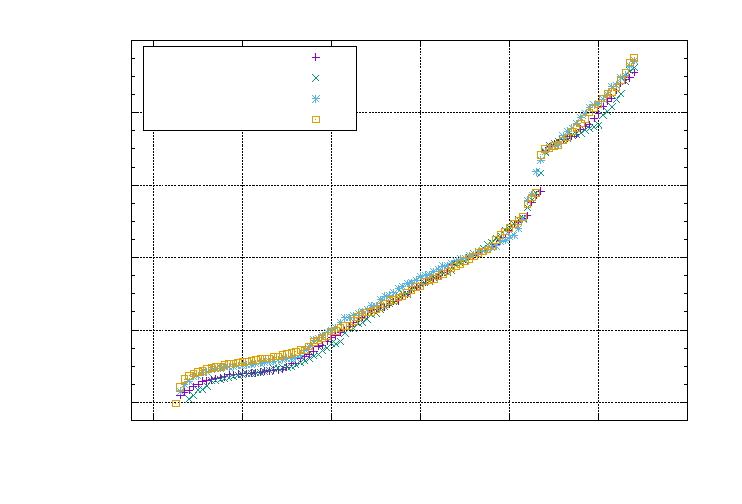
\includegraphics{kovegenv}}%
    \gplfronttext
  \end{picture}%
\endgroup

    \caption{Egenvärden till kovariansmatrisen från \eqref{eq:C} för fyra olika strängar. Det största egenvärdent ses vara åtminstone $10^{16}$ storlekar större än det minsta, vilket påvisar en signifikant skillnad i bidrag till rörelsen från vardera egenmod.}
    \label{fig:kovegenvarde}
\end{figure}



\begin{figure}
    \centering
    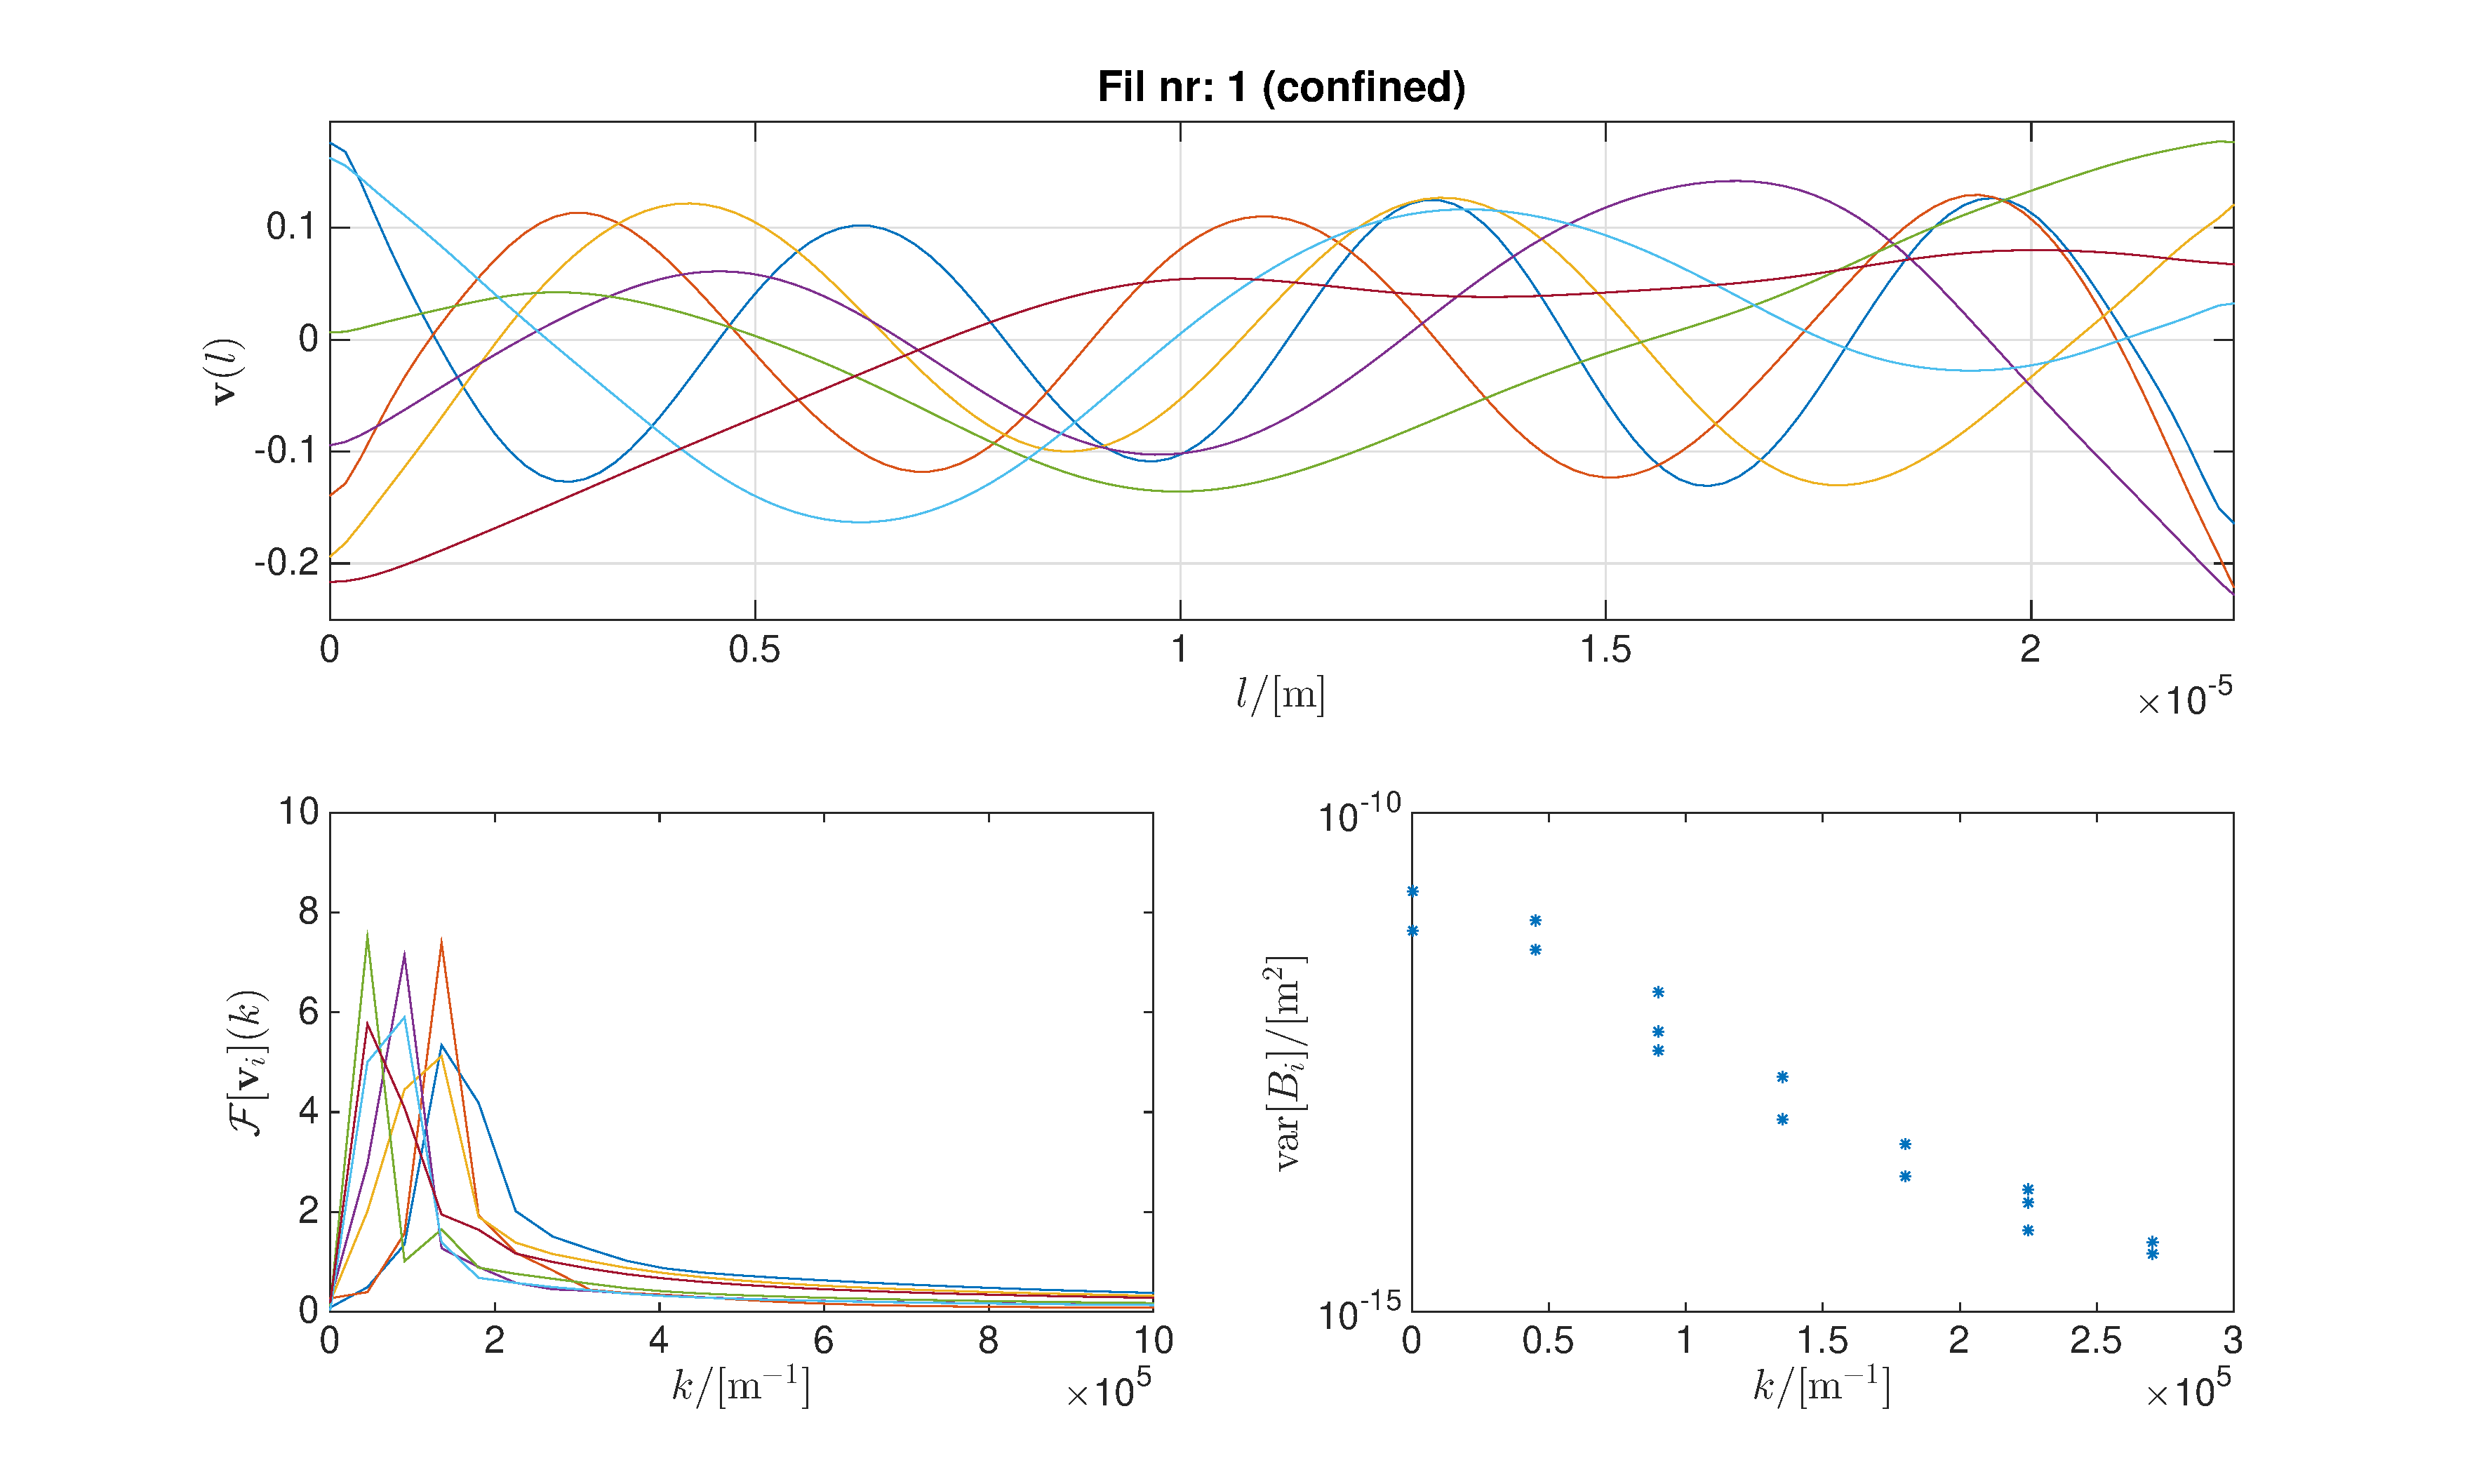
\includegraphics[width=\textwidth]{egenmoder.eps}
    \caption{Caption}
    \label{fig:egenmoder}
\end{figure}

%Resultat som kan tas med

%Motivera att jämviktsläge fanns
%Uppdelningen i egenmoder, olika relaxationstid
%Dispersionsrelation?
%Skillnad mellan confined och unconfined



\section{Diskussion}




%Bara en liten kodsnutt som behövs när man kompilerar lokalt
%%% Local Variables: 
%%% mode: latex
%%% TeX-master: "00main.tex"
%%% End: 